%
% CHAPTER: Preliminaries
%

\chapterimage{Koenigsberg_Map_by_Bering_1613.pdf} % Chapter heading image

\chapter{Discrete Mathematics}
\label{chap:Discrete_Mathematics}

\begin{quote}
\begin{flushright}
\emph{Mathematics may be defined as the subject in which\\
we never know what we are talking about,\\
nor whether what we are saying is true.}\\
Bertrand Russell
\end{flushright}
\end{quote}
\bigskip

Most of the mathematics used throughout this book belong to the area of \emph{discrete mathematics}. Discrete mathematics is characterized because it studies mathematical objects that have distinct or separated values, rather than continuous. Examples of discrete objects used in this book are integers, strings, graphs and computer programs. A key distinctive element of discrete sets is that they can be enumerated with natural numbers, that is, they are countable. We will barely use continuous mathematics, for example calculus, in the theoretical developments of the theory of nescience.

Our main interest in discrete mathematics is because computers. The theory of nescience borrows concepts and ideas from multiple areas of computer science: algorithms, coding, string complexity and others. Computers operate in discrete steps and the data processed is stored in discrete units of memory. We are interested in computers because we want to apply our theoretical developments to as many real objects as possible, and we think that the right way to model our world is by means of using computers. In pure mathematics it is customary to discuss abstract objects without worrying about what they represent. In the theory of nescience, on the contrary, the representation (encoding) of objects plays a crucial role.

This chapter is intended as a quick review of the basic concepts of discrete mathematics; no formal definitions are provided and theorems are not proved. Discrete mathematics is an extremely diverse and large area of study. We will review only those elements that are required to understand the theory of nescience. Some of the theories involved (computability, information, complexity, ...) require a deeper coverage, and so, they are studied in separate chapters. In the References section there is a list of suggested books that explain in detail the topics covered in this chapter.

%
% Section: Sets
%

\section{Sets, Relations and Functions}
\label{sec:sets}

The sets of \emph{natural}\index{Set of natural numbers}, \emph{integers}\index{Set of integers}, \emph{rational}\index{Set of rationals}, and \emph{real}\index{Set of real numbers} numbers are represented by $\mathbb{N}$, $\mathbb{Z}$, $\mathbb{Q}$, and $\mathbb{R}$ respectively, which includes the number $0$. The \emph{positive integers}\index{Set of positive integers} are denoted by $\mathbb{Z}^+$, and the \emph{positive reals}\index{Set of positive reals} by $\mathbb{R}^+$, where both of these sets incorporate the number $0$. Let $A$ be a \emph{set}\index{Set}. We signify that $x$ is an \emph{element}\index{Element of a set} of $A$ by the notation $x\in A$, and that $x$ is not an element of $A$ by $x \notin A$. Elements of a set can be enumerated using braces, such as $A = \{0, 1, 2, 3\}$, or they can be defined by conditions via the \emph{set-builder}\index{Set formation notation} notation, for instance $A = \{x \in \mathbb{N} : x < 4\}$, with the stipulation that the \emph{universe}\index{Universe of a set} of the set be clearly established.

Suppose $A$ and $B$ are two sets. We use the notation $A = B$ to denote that the sets are \emph{equal}\index{Equal sets}. The expression $A \subseteq B$ signifies that $A$ is a \emph{subset or equal}\index{Subset} to $B$, and $A \subset B$ is used to indicate that $A$ is a \emph{proper subset}\index{Proper subset} of $B$ (implying $A$ is not equivalent to $B$). The condition $A = B$ holds true if, and only if, both $A \subseteq B$ and $B \subseteq A$ are satisfied concurrently. The symbol $\varnothing$ represents the \emph{empty set}\index{Empty set}, a set that contains no elements.

\begin{example}
For every set $A$ we have that $\varnothing \subseteq A$ and $ A \subseteq A$.
\end{example}

The term \emph{cardinality}\index{Cardinality of a set} refers to the number of elements within a finite set $A$, denoted as $d(A)$. Accordingly, the cardinality of the empty set $\varnothing$ is 0, as it contains no elements. For any two sets $A$ and $B$, the notation $A \cup B$ signifies the \emph{union}\index{Union of sets} of $A$ and $B$, whereas $A \cap B$ designates the \emph{intersection}\index{Intersection of sets} of $A$ and $B$. When dealing with $n$ sets, say $A_1, A_2, \ldots, A_n$, their union and intersection are denoted as $\cup_{i=1}^n A_i$ and $\cap_{i=1}^n A_i$ respectively. For an arbitrary collection of sets indexed by $I$, we employ $\cup_{i \in I} A_i$ and $\cap_{i \in I} A_i$. In the context of an infinite collection of sets, the notations $\cup_{i}^{\infty} A_i$ and $\cap_{i}^{\infty} A_i$ are adopted.

On occasion, we will resort to the use of \emph{Venn diagrams}\index{Venn diagram} as a visual means to represent sets, as exemplified in Figure \ref{fig:Venn-diagram}.

\begin{figure}[t]
\centering
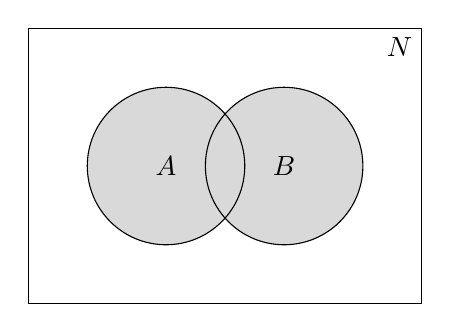
\begin{tikzpicture}

    % Rectangle with label
    \draw (0,0) rectangle (5,3.5) node[below left] {$\mathbb{N}$};
    
    \fill[gray!30] (1.75,1.75) circle (1);
    \fill[gray!30] (3.25,1.75) circle (1);

    \node[draw, circle, minimum width=2cm, label=center:{$A$}] at (1.75, 1.75) {};
    \node[draw, circle, minimum width=2cm, label=center:{$B$}] at (3.25, 1.75) {};

\end{tikzpicture}
\caption{\label{fig:Venn-diagram}Representation of $A \cup B$ as a Venn Diagram}
\end{figure}


Given the sets $A$ and $B$, $A \backslash B$ is the \emph{set difference}\index{Set difference}, and ${A}^c$ is the \emph{complement}\index{Complement of a set} set of $A$. The \emph{De Morgan's laws}\index{De Morgan's laws} state that for every two sets $A$ and $B$ we have that $\left( A \cup B \right)^c = A^c \cap B^c$ and $\left( A \cap B \right)^c = A^c \cup B^c$.

Two sets $A$ and $B$ are \emph{disjoint}\index{Disjoint sets} if $A \cap B = \varnothing$. The sets $A_1, A_2, \ldots, A_n$ are disjoint if for every $i$ and $j$ such that $i \neq j$ we have that $A_i \cap A_j = \varnothing$. A \emph{partition}\index{Partition of a set} of a set $A$ is a collection of nonempty disjoint subsets of $A_1, A_2, \dots, A_n$ of $A$ such that  $A = \cup_{i=1}^n A_i$. The \emph{power set}\index{Power set} $\mathcal{P}(A)$ is the set whose members are all possible subsets of A. If $d(A)=n$ then $d\left( \mathcal{P}(A) \right) = 2^n$.

Given any two sets $A$ and $B$, we denote the \emph{set difference}\index{Set difference} as $A \backslash B$, and the \emph{complement}\index{Complement of a set} of the set $A$ as ${A}^c$. \emph{De Morgan's laws}\index{De Morgan's laws} articulate that for any pair of sets $A$ and $B$, we have $\left( A \cup B \right)^c = A^c \cap B^c$ and $\left( A \cap B \right)^c = A^c \cup B^c$.

The term \emph{disjoint}\index{Disjoint sets} is applied to two sets $A$ and $B$ when their intersection $A \cap B = \varnothing$. We say that the sets $A_1, A_2, \ldots, A_n$ are disjoint if for every distinct pair $i$ and $j$ ($i \neq j$), we find $A_i \cap A_j = \varnothing$. A \emph{partition}\index{Partition of a set} of a set $A$ is an assembly of nonempty disjoint subsets $A_1, A_2, \dots, A_n$ of $A$ satisfying  $A = \cup_{i=1}^n A_i$. The \emph{power set}\index{Power set} of $A$, denoted as $\mathcal{P}(A)$, is the collection of all conceivable subsets of $A$. If the cardinality of $A$ is $n$, i.e., $d(A)=n$, then the cardinality of the power set of $A$ is $2^n$, thus expressed as $d\left( \mathcal{P}(A) \right) = 2^n$.

\begin{example}
Given the set $A = \{1, 2, 3\}$, its power set is:
\[
\mathcal{P}(A) = \{\varnothing, \{1\}, \{2\}, \{3\}, \{1,2\}, \{1,3\}, \{2,3\}, A\}
\]
\end{example}

Consider a non-empty set $A$ and a collection $\mathcal{F}$ of subsets of $A$. The pair $\left( A, \mathcal{F} \right)$ is designated as an \emph{field}\index{Field of sets} over $A$ if it fulfills the following conditions: it includes the empty set, denoted as $\varnothing \in \mathcal{F}$, it is closed under the operation of complementation, meaning for each $F \in \mathcal{F}$, the complement $F^c  \in \mathcal{F}$, and it is closed under finite unions, which indicates $F_1 \cup \ldots \cup F_n  \in \mathcal{F}$ for all subsets $F_1, \ldots, F_n \in \mathcal{F}$. Additionally, it can be demonstrated that a field also fulfills two further criteria: $A \in \mathcal{F}$, and it is closed under finite intersections, expressed as $F_1 \cap \ldots \cap F_n  \in \mathcal{F}$ for all subsets $F_1, \ldots, F_n \in \mathcal{F}$.

% Relations

Consider two elements, $x$ and $y$. An \emph{ordered pair}\index{Ordered pair}, symbolized as $(x, y)$, is a pairing of $x$ and $y$ in that order. By expanding this concept, an \emph{n-tuple}\index{n-tuple} — which can be visualized as an $n$-element ordered pair — is written as $(x_1, \ldots, x_n)$. We define the \emph{Cartesian product}\index{Cartesian product} of two sets $A$ and $B$, which is symbolized as $A \times B$. This product is a set consisting of all possible ordered pairs $(x, y)$, where $x$ belongs to set $A$ and $y$ belongs to set $B$. The Cartesian product can be extended to $n$ sets, $A_1, A_2, \dots, A_n$, and is expressed as $A_1 \times A_2 \times \dots \times A_n$. Moreover, the \emph{n-fold Cartesian product} of a set $A$ with itself is represented as $A^n$.

Let $R$ be a subset of the Cartesian product of set $A$ with itself, i.e., $R \subseteq A \times A$. Such a subset is referred to as a \emph{binary relation}\index{Binary relation}, which can be represented as $aRb$, meaning that the ordered pair $(a, b)$ is a member of $R$. A binary relation is deemed \emph{reflexive}\index{Reflexive relation} if for any element $a$ in $A$, it holds that $aRa$. It is termed \emph{symmetric}\index{Symmetric relation} if for all $a, b$ in $A$, the presence of $aRb$ automatically implies $bRa$. The property of \emph{antisymmetric}\index{Antisymmetric relation} is attributed to a binary relation when the coexistence of $aRb$ and $bRa$ leads to the conclusion that $a = b$. It is considered \emph{transitive}\index{Transitive relation} if for any $a, b, c$ in $A$, the occurrence of $aRb$ and $bRc$ infers $aRc$. A binary relation is identified as \emph{total}\index{Total relation} if for all $a, b$ in $A$, either $aRb$ or $bRa$ holds. Binary relations can be extended to include two different sets $A$ and $B$ as a subset $R \subseteq A \times B$, and can also be adapted to \emph{n-ary} relations represented as $R \subseteq A_1 \times A_2 \times \dots \times A_n$.

Let $R$ be a binary relation that is a subset of the Cartesian product $A \times A$, i.e., $R \subseteq A \times A$. If this relation is reflexive, symmetric, and transitive, it is designated as an \emph{equivalence relation}\index{Equivalence relation}, typically symbolized by $\sim$. Within the context of an equivalence relation, two elements $a, b$ from set $A$ are deemed \emph{equivalent}\index{Equivalent elements} if the relation $a \sim b$ holds. The notion of an \emph{equivalence class}\index{Equivalence class}, denoted as $[a]$, refers to the set of all elements in $A$ that are equivalent to a particular element $a$. In other words, the equivalence class of $a$ is defined as $[a] := \{ b \in A : a \sim b\}$. An equivalence relation serves to partition the base set into what is known as the \emph{quotient set}\index{Quotient set}. Represented as $A / {\mathord {\sim }}$, the quotient set consists of all equivalence classes stemming from elements of $A$, that is, $A / {\mathord {\sim }} := \{ [a] : a \in A \}$.

A binary relation that is reflexive, transitive, and antisymmetric is known as a \emph{partial order}\index{Partial order}, often represented by the symbol $\preceq$. A set equipped with a partial order is referred to as a \emph{partially ordered set}\index{Partially ordered set}, also abbreviated as \emph{poset}\index{poset}. In the context of a poset, an element $a$ from set $A$ is considered \emph{minimal}\index{Minimal element} if there is no other element $b$ in $A$ for which $b \preceq a$. Similarly, an element $a$ is labeled as \emph{maximal}\index{Maximal element} if no other element $b$ in $A$ exists such that $a \preceq b$. A relation that embodies reflexivity, transitivity, antisymmetry, and totality is designated as a \emph{total order}\index{Total order}, typically symbolized by $\leq$. A set that is coupled with a total order is identified as a \emph{totally ordered set}\index{Totally ordered set}. For any totally ordered set $A$, the \emph{maximum}\index{Maximum element} element is represented by $\max(A)$, meaning that $\max(A) \geq x$ holds for all $x$ in $A$. Similarly, the \emph{minimum}\index{Minimum element}, represented by $\min(A)$, is defined as an element such that $\min(A) \leq x$ for all $x$ in $A$.

\begin{example}
Let $R$ be a relation that is a subset of the Cartesian product of the set of natural numbers $\mathbb{N}$ with itself, i.e., $R \subset \mathbb{N} \times \mathbb{N}$. In this relation, an ordered pair $(a, b)$ belongs to $R$ if $a$ is a divisor of $b$. The set $\mathbb{N}$, when paired with relation $R$, forms a partially ordered set. In this context, the number $11$ serves as a minimal element of $R$. This is because $11$ is a prime number, which, by definition, can only be divided evenly by 1 and itself.
\end{example}

% Functions

A \emph{function}\index{Function} is defined as a binary relation $f \subseteq A \times B$, where for each element $x \in A$, there exists at most one $y \in B$ satisfying the condition $\left(x, y\right) \in f$. In this context, elements $\left(x, y\right) \in f$ are denoted by $f(x)=y$, with the function represented by $f : A \rightarrow B$. The set $A$ is referred to as the \emph{domain}\index{Domain} of $f$, and $B$ is the \emph{codomain}\index{Codomain}. The set $\{ y \in B : \exists x \in A , f(x) = y\}$ constitutes the \emph{range}\index{Range} of $f$. If the relation is not defined for all $x \in A$, the function is termed \emph{partial}\index{Partial function}, denoted by $f(x) \uparrow$ for undefined $x$ in the function $f$. 

\begin{example}
In Section \ref{sec:computable_functions}, we will discuss an alternate interpretation of a function as a procedure, or a series of steps, that assigns an element of $B$ to each element of $A$. For instance, the subsequent C code delineates a partial function from $\mathbb{R}$ to $\mathbb{R}$, characterized as partial due to $inv(0)\uparrow$:
\begin{verbatim}
    double inv(double x) {
        return 1 / x;
    }
\end{verbatim}
\end{example}

A function is said to be \emph{injective}\index{Injective function} if, for all elements $x$ and $y$, $f(x) = f(y)$ implies $x=y$. A function is \emph{surjective}\index{Surjective function} when for every $y$, there exists at least one $x$ such that $f(x) = y$. A function is described as \emph{bijective}\index{Bijective function} if it exhibits both injective and surjective properties. The \emph{identity}\index{Identity function} function $I_A : A \rightarrow A$, determined by $f(a) = a$ for all $a \in A$, is bijective. These concepts of function, partial function, injective, surjective, and bijective can be extended to $n$-ary functions, represented as $f: A_1 \times A_2 \times \dots A_n \rightarrow B$.

The \emph{inverse}\index{Inverse function} function of a function $f$, represented by $f^{-1}$, is identified by $f(f^{-1}(x)) = f^{-1}(f(x)) = x$. Given two functions $f$ and $g$, where the domain of $f$ coincides with the range of $g$, we define the \emph{composition}\index{Composition} of $f$ with $g$, represented by $f \circ g$, as $f \circ g = f(g(x))$.

An infinite set $A$ is designated as \emph{countable}\index{Countable set} if there is a bijective function that maps the elements of $A$ onto the set of natural numbers $\mathbb{N}$. In contrast, a set is deemed \emph{uncountable}\index{Uncountable set} if it is not finite and also not countable. We refer to a set as having \emph{countably many}\index{Countably many set} elements if it is either finite or countable.

\begin{example}
Sets like $\mathbb{N}$, $\mathbb{Z}$ and $\mathbb{Q}$ are countable, while $\mathbb{R}$ is not.
\end{example}

The \emph{characteristic function}\index{Characteristic function} of a set $A$ is denoted as $1_A : A \rightarrow \{1, 0\}$, where $1_A(x) = 1$ if $x \in A$ and $0$ otherwise.

Considering a real number $x \in \mathbb{R}$, its \emph{absolute value}\index{Absolute value}, represented as $\mid x \mid$, is defined to be $x$ if $x \geq 0$ and $-x$ if $x < 0$. The \emph{ceil}\index{Ceil} function of $x$, denoted as $\lceil x \rceil$, is the smallest integer that is greater than or equal to $x$. The \emph{floor}\index{Floor} function of $x$, represented by $\lfloor x \rfloor$, is the largest integer that is less than or equal to $x$. Given two positive integers $a$ and $b$, the \emph{modulo}\index{Modulo} operation of $a$ and $b$, symbolized by $a \bmod b$, gives the remainder of the integer division of $a$ by $b$.

For two functions $f$ and $g$, defined as $f,g:\mathbb{N}\rightarrow\mathbb{R}^{+}$, we assert that $f(n)$ is of \emph{order of}\index{Order of a function} $g(n)$, symbolized by $f(n)=O(g(n))$, if there exist positive integers $c$ and $m$ such that $f(n)\leq cg(n)$ for every integer $n \geq m$. If $f(n)=O(g(n))$, we denote $g$ as an \emph{upper bound}\index{Upper bound of a function} for $f$.

%
% Section: Strings and Languages
%

\section{Strings and Languages}
\label{sec:strings}

Let $\mathcal{S}=\left\{ s_{1},s_{2},\ldots,s_{q}\right\}$ be a non-empty finite set called \emph{alphabet}\index{Alphabet}, whose elements are called \emph{symbols}\index{Symbols}. A \emph{sequence}\index{Sequence of symbols} over $\mathcal{S}$ is any ordered collection of symbols $x_1 x_2 \dots x_n$ from $\mathcal{S}$. When the alphabet is the set $\mathcal{B} = \{0, 1\}$, the sequences are called \emph{binary}\index{Binary sequence}. If the sequence is finite we call it \emph{string}\index{String}. In this book we will be working mostly with binary strings. The \emph{length}\index{Length of a string} of a string $s$, denoted by $l(s)$, is the number of symbols in $s$. The \emph{empty string}\index{Empty string} is the unique string over $\mathcal{S}$ of length 0, and is denoted $\lambda$. Let $x \in \mathcal{S}$, by $x^n$ we denote the string $x x \ldots x$ ($n$-times). If $s = x_1 x_2 \dots x_n$ is a string, its \emph{reverse}\index{Reverse string} $s^R$ is $x_n x_{n-1} \dots x_1$.

Let $\mathcal{S}^{n}$ denote the set of all strings $s_{1}s_{2}\ldots s_{n}$ of length $n$\footnote{Do not confuse the set of strings of length $n$ over an alphabet $\mathcal{S}^n$ with the $n$-fold Cartesian product of a set $S^n$, alphabets will be represented by using calligraphic fonts.}, $\mathcal{S}^{+}=\cup_{n\geq1}\mathcal{S}^{n}$ and $\mathcal{S}^{\ast} = \mathcal{S}^{+} \cup \{\lambda\}$. Note that all the strings that belong to $\mathcal{S}^{\ast}$ have finite lengths. $\mathcal{S}^{\ast}$ is called the \emph{Kleene closure}\index{Kleene closure} of $\mathcal{S}$.

\begin{example}
The following relations hold: $d \left( \left\{ s \in \mathcal{B}^{\ast} : l(s) = n \right\} \right) = 2^n$ and $d \left( \left\{ s \in \mathcal{B}^{\ast} : l(s) \leq n \right\} \right) = 2^{n+1}-1$.
\end{example}













For any two strings $s$ and $t$ in $\mathcal{S}^{\ast}$, the \emph{concatenation}\index{String concatenation} of $s$ and $t$, denoted by $st$, is defined as the sequence of symbols in $s$ followed by the sequence of symbols in $t$. Note note that $l(st) = l(s) + l(t)$. $S^\ast$ is closed under the operation of concatenation. $S^\ast$ with the operation of concatenation forms a \emph{free monoid}, that it, it is associative  $s(tr)=(st)r$, and has an identity element $\lambda a = a \lambda = a$.

A string $s$ is said to be a \emph{substring}\index{Substring} of $t$ if there exist (possibly empty) strings $u$ and $v$ such that $t$ = $usv$. A string $s$ is said to be a \emph{prefix}\index{Prefix string} of $t$, denoted by $s <_p t$, if there exists a string $u$ such that $t = su$. A subset $S \subset \mathcal{S}^{\ast}$ is \emph{prefix free}\index{Prefix free set} if for all $s, t \in S$, if $s <_p t$ then $s = t$. Given a string $s \in \mathcal{S}^{\ast}$, the \emph{self delimited}\index{Self delimited string} version of $s$, denoted by $\bar{s}$, is $\bar{s} = 1^{l(s)}0s$. Note that $l(\bar{s}) = 2l(s)+1$.

\begin{example}
The set $\bar{\mathcal{S}^{\ast}}$composed by all the self delimited strings of $\mathcal{S}^{\ast}$ is prefix free.
\end{example}

If $\mathcal{S}$ is a total ordered set, we can define a total order on $\mathcal{S}^{\ast}$, called \emph{shortlex ordering}\index{Shortlex ordering}, in which sequences are primarily sorted by length with the shortest sequences first, and sequences of the same length are sorted into their lexicographical order.

\begin{example}
If $S = \{a, b, c\}$ and $a < b < c$, then the shortlex order on $\mathcal{S}^{\ast}$ includes the relations $\lambda < a < b < c < aa < ab < \ldots < cc < aaa < aab < \ldots < ccc < \ldots$
\end{example}

Given an arbitrary object $O$ we denote its representation as a string as $\left\langle O\right\rangle$, assuming that there exists an standard encoding method. Given the objects $O_{1},O_{2},\ldots,O_{k}$, the concatenation of the representations of these objects $\left\langle O_1 \right\rangle \left\langle O_2 \right\rangle \ldots \left\langle O_k \right\rangle$ is denoted by $\left\langle O_1 O_2 \ldots O_k \right\rangle$. The concatenation of the representation of these objects in such a way that we can decode and uniquely identify all of them is represented by $\left\langle O_1, O_2,\ldots,O_k \right\rangle$, for example, we could use $\left\langle O_1, O_2,\ldots,O_k \right\rangle = \bar{\left\langle O_1 \right\rangle} \bar{\left\langle O_2 \right\rangle} \ldots \bar{\left\langle O_k \right\rangle}$.

\begin{example}
Natural numbers can be represented by binary strings using the following encoding method: $\langle 0 \rangle = \lambda$, $\langle 1 \rangle \rightarrow 0$, $\langle 2 \rangle \rightarrow 1$, $\langle 3 \rangle \rightarrow 00$, $\langle 4 \rangle \rightarrow 01$, $\langle 5 \rangle \rightarrow 10$, $\langle 6 \rangle \rightarrow 11$, $7 \rightarrow 000$, ... The pair of numbers $\left\langle 3, 7 \right\rangle$ would be represented as $110001110000$. Given this encoding we have that $l \left( \langle n \rangle \right) = \lfloor \log_2 (n + 1) \rfloor$.
\end{example}

A \emph{language}\index{Language} $L$ over an alphabet $\mathcal{S}$ is a subset of strings $L \subset \mathcal{S}^{\ast}$. The elements of $L$ are called \emph{words}\index{Words of a language}. The \emph{empty language}\index{Empty language} is the language that contains no words $L = \varnothing$. 

Let $L_1$ and $L_2$ be two languages over an alphabet $\mathcal{S}$. Common operations over languages include language concatenation $L_1 \cup L_2 = \{ w \in \mathcal{S}^{\ast} \mid w \in L_1 \lor w \in L_2 \}$, language intersection $L_1 \cap L_2 = \{ w \in \mathcal{S}^{\ast} \mid w \in L_1 \land w \in L_2 \}$, language complement $\lnot L_1 = \{ w \in \mathcal{S}^{\ast} \mid w \notin L_1 \}$, and Kleen closure $L_1^\ast = \{ \lambda \} \cup \{ wz \mid w \in L_1 \land z \in L_1^\ast \}$. 

Languages can be axiomatically generated by using finite collections of rules for string rewriting called grammars. A \emph{grammar}\index{Grammar} $G$ is a tuple $(N, \Sigma, P, S)$ composed by: a finite set $N \subset \mathcal{S}$ of \emph{nonterminal symbols}\index{Non-terminal symbol}; a finite set $\Sigma \subset \mathcal{S}$ of \emph{terminal symbols}\index{Terminal symbol}; and a finite set $P$ of \emph{production rules}\index{Production rule} in the form $( \Sigma \cup N )^\ast N ( \Sigma \cup N) \rightarrow (\Sigma \cup N)^\ast$; and a \emph{start symbol}\index{Start symbol} $S \in N$. Each production rule maps from one string of symbols to another, beginning with the start symbol.

\begin{example}
\label{ex:context_free_grammar}
Given the alphabet $\mathcal{S} = \{ S, a, b \}$ we define the grammar $(N, \Sigma, P, S)$, whre $N = \{ S \}$, $\Sigma = \{ a, b \}$, $P = \{ S \rightarrow aSb, S \rightarrow ba \}$, and the start symbol $S \in N$. This grammar produce the language $L = \{ a^nbab^n \mid n\geq0 \} = \{ ba, abab, aababb, aaababbb, \ldots \}$.
\end{example}

\emph{Chomsky hierarchy}\index{Chomsky hierarchy} is a classification of grammars according to their expressive power, that is, the type of languages they can generate. From more restrictive to less restrictive grammars, we have ($a$ is a terminal symbol, $A, B$ are non-terminal symbols, and $\alpha, \beta$ and $\gamma$ are strings of terminal or non-terminal symbols):

\begin{description}
\item[Type-3] or \emph{regular grammars}\index{Regular grammar}, in which the left-hand side of each production rule consists of only a single nonterminal symbol, and the right-hand side may be the empty string, a single terminal symbol, or a single terminal symbol followed by a nonterminal symbol ($A \rightarrow \lambda$, $A \rightarrow a$, $A \rightarrow aB$).

\item[Type-2] or \emph{context-free grammar}\index{Context-free-grammar}, in which the left-hand side of each production rule consists of only a single nonterminal symbol ($A \rightarrow \alpha$). 

\item[Type-1] or \emph{context sensitive grammar}\index{Context sensitive grammar}, in which the left-side and right-side of the production rules may be surrounded by a context of terminal and nonterminal symbols ($\alpha A \beta \rightarrow \alpha \gamma \beta$).

\item[Type-0] or \emph{recursively enumerable grammar}\index{Recursively enumerable grammar}, in which there are no constrains to the production rules ($\gamma \rightarrow \alpha$).
\end{description}

\begin{example}
The grammar of Example \ref{ex:context_free_grammar} is of Type-2 context-free.
\end{example}

The \emph{Backus–Naur form}\index{Backus–Naur form} is a notation for context-free grammars that is commonly used in computer science to formally describe the syntax of programming languages and communication protocols. A Backus–Naur form is a set of production rules with the following format

\begin{verbatim}
    <symbol> ::= __expression__
\end{verbatim}

where \texttt{<symbol>} is a non-terminal symbol, \texttt{\_\_expression\_\_} is a string of terminal or non-terminal symbols, and \texttt{::=} means that the symbol on the left must be replaced with the expression on the right. Multiple  \texttt{\_\_expression\_\_} can be combined in a single production rule by separating them with the vertical bar \texttt{|}, meaning that we can choose any of them for the replacement. Symbols that never appear on a left side of a production rule are terminals. Symbols that appear on a left side are non-terminals; non-terminal symbols are always enclosed between the pair \texttt{<>}. The non-terminal symbol of the first production rule is considered the starting symbol.

\begin{example}
The grammar of Example \ref{ex:context_free_grammar} can be expressed in Backus-Naur form with the following production rule:
\begin{verbatim}
    <string> ::= a <string> b | ba
\end{verbatim}
\end{example}

%
% Section: Graphs
%

\section{Graphs}
\label{sec:Graphs}

A \emph{graph}\index{Graph}\footnote{The definition of graph provided in this introduction is equivalent to the definition of \emph{simple graph} in the standard discrete mathematics literature.} $G$ is an ordered pair $(V,E)$ composed by a nonempty set of objects $V$, called \emph{vertices}\index{Vertices of a graph}, connected by set of links $E$, called \emph{edges}\index{Edges of a graph}. The elements of $E$ have the form of unordered pairs $\left\{ u,v\right\}$ of distinct (no loops allowed) vertices $u$,$v\in V$. Vertices $u$ and $v$ are said to be \emph{adjacent}\index{Adjacent vertices} if there is and edge $\left\{ u,v\right\} \in E$, and if so, they are called the \emph{endpoints}\index{Endpoints of an edge} of the edge. If the set $V$ is infinite, the graph is called \emph{infinite graph}\index{Infinite graph}; in this book we will consider only finite graphs. If $G = (V,E)$ is a graph, its \emph{adjacency matrix}\index{Adjacency matrix} is a square $d(V) \times d(V)$ matrix $A$ such that the element $A_{uv}$ is 1 if $\left\{ u,v\right\} \in E$ and 0 otherwise.

Graphs are usually depicted as a set of dots for the vertices, joined by lines for the edges.

\begin{example}
\label{ex:binary_tree}
Let $V=\{a, b, c, d\}$ and $E=\{ \{a,b\}, \{a,c\}, \{a,d\}, \{b,c\} \}$, the graph $G=(V,E)$ is depicted in Figure \ref{fig:Graph-Example}.
\end{example}

\begin{figure}[h]
\centering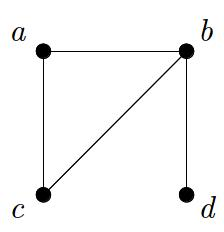
\includegraphics[scale=0.5]{GraphExample}
\caption{\label{fig:Graph-Example}An Example of Graph}
\end{figure}

If $v$ is an endpoint of and edge $e$, then we say that $e$ is is \emph{incident}\index{Incident edge} on $v$. The \emph{degree}\index{Degree of a vertex} of a vertex $v$, written $\deg(v)$, is equal to the number of edges which are incident on $v$. A vertex of degree zero is called \emph{isolated}\index{Isolated vertex}; a vertex of degree one is called \emph{pendant}\index{Pendant vertex}. The \emph{neighborhood}\index{Neighborhood of a vertex} of vertex $v$, denoted by $N(v)$, is the set of all vertices that are adjacent to $v$. If $A \subset V$, the neighborhood of $A$ is $N(A) = \cup_{v \in A} N(v)$. A \emph{path}\index{Path} in a graph is a sequence of distinct vertices $\{v_{0}, v_{1}, \ldots ,v_{k}\}$ in which $v_{i}$ and $v_{i+1}$ are adjacent for each $1 \leq i < k$. A path is a \emph{simple path}\index{Simple path} if it does not repeat any node. A graph is \emph{connected}\index{Connected graph} if every two nodes have a path between them. If $v_{0} = v_{k}$ we say that the path is a \emph{cycle}\index{Cycle}. A cycle is a \emph{simple cycle}\index{Simple cycle} if it contains at least three nodes and repeats only the first and last nodes. 

\begin{example}
Given a graph $G=(V,E)$, the \emph{handshaking theorem}\index{Handshaking theorem} states that $\sum_{v \in V} deg(v) = 2 m$, where $m = d(E)$, since each edge has two end points.
\end{example}

If the pairs of vertices $u, v$ are ordered pairs, the graph is called \emph{directed graph}\index{Directed graph}, and in that case, $u$ is called the \emph{initial vertex}\index{Initial vertex} and $v$ the \emph{terminal vertex}\index{Terminal vertex}. If $G$ is directed graph, we call the \emph{in-degree}\index{In-degree of a vertex} of a vertex $v$, denoted by $indeg(v)$, to the number of edges in which $v$ is an terminal vertex, and \emph{out-degree}\index{Out-degree of a vertex}, denoted by $outdeg(v)$, to the number of edges in which $v$ is an initial vertex. A directed grap is \emph{strongly connected}\index{Strongly connected graph} is a direct path connects every two nodes. Directed graphs are depiced using arrows instead of lines to represent edges.

A graph $G$ is said to be \emph{bipartite}\index{Bipartite graph} if the set of vertices $V$ can be partitioned into two subsets $V_1$ and $V_2$ such that each edge of $G$ connects a vertex of $V_1$ to a vertex of $V_2$. Bipartite graphs are usually denoted by $G=(V_1, V_2, E)$. The degree of the vertices of a bipartite graph satisfied the following property, called the \emph{degree sum formula}\index{Degree sum formula}, $\sum_{u \in V_1} deg(u) = \sum_{v \in V_2} deg(v) = d(E)$.

A graph $G(V',E')$ is a \emph{subgraph}\index{Subgraph} of $G(V,E)$ if $V'$ is a subset of $V$ and $E'$ is a subset of $E$ whose endpoints belong to $V'$. A graph $G$ is called a \emph{labeled graph}\index{Labeled graph} if its edges and/or vertices are assigned data of one kind or another. In particular, if each edge $e$ of $G$ is assigned a nonnegative number $w(e)$ then $w(e)$ is called the \emph{weight}\index{Weight of an edge} of $e$.

A particular type of graph that will be extensively used in this book are trees. A \emph{tree}\index{Tree} is a non-empty graph in which any two vertices are connected by a unique path. Given a tree, we will always designate a particular vertex, called the \emph{root}\index{Root of a tree} of the tree, and direct each edge away from that root.

\begin{example}
An equivalent definition of trees is provided by set theory. According to set theory a tree is a partially ordered set $(T, <)$ such that for each $t \in T$, the set $S = \{ s \in T : s < t \}$ has an element that is smaller than every other element of S (\emph{least element}).
\end{example}

Let $T$ be a tree. If $v$ is a vertex in $T$ other than the root, the \emph{parent}\index{Parent of a vertex} of $v$ is the unique vertex $u$ such that there is an edge connecting $u$ to $v$. If $u$ is the parent of $v$, then $v$ is called a \emph{child}\index{Child of a vertex} of $u$. A \emph{sibling}\index{Sibling to a vertex} to a vertex $v$ is any other vertex on the tree which has the same parent than $v$. The \emph{ancestors}\index{Ancestors of a vertex} of a vertex are the vertices in the path from the root to this vertex, excluding the vertex itself and including the root. The \emph{descendants}\index{Descendant of a vertex} of a vertex $v$ are those vertices that have $v$ as an ancestor. A vertex is called a \emph{leaf}\index{Leaf vertex} if it has no children. Vertices that have children are called \emph{branches}\index{Branches of a tree}. The \emph{depth}\index{Depth of a vertex} of a vertex $v$ is the length of the unique path from the root to $v$. The \emph{height}\index{Height of a tree} of a tree is the maximum of the levels of its vertices. 

\begin{example}
The following applies to the tree depicted in Figure \ref{fig:BinaryTree-Example}: the root is the vertex $a$; $c$ is a parent of $d$ and $d$ is a child of $c$; $d$ and $g$ are siblings; the ancestors of $d$ are $a$ and $c$; the descendants of $c$ are $e$, $e$ and $f$; $b$, $e$, $f$ and $g$ are leaf nodes; $c$ and $d$ are branches; the depth of $d$ is 3; the height of the tree is 4.
\end{example}

\begin{figure}[h]
\centering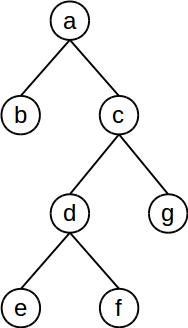
\includegraphics[scale=0.5]{BinaryTree}
\caption{\label{fig:BinaryTree-Example}An Example of Tree}
\end{figure}

If $v$ is a vertex in a tree, the \emph{subtree}\index{Subtree} with $v$ as root is the subgraph of the tree consisting of $v$ and its descendants and all edges incident to these descendants. A tree is called an \emph{k-ary tree}\index{k-ary tree} if every branch has not more than $k$ children. The tree is called a \emph{full k-ary tree}\index{full k-ary tree} if every branch has exactly $k$ children. An \emph{k-ary} tree with $k=2$ is called a \emph{binary tree}\index{Binary tree}. A $k$-ary tree of height $h$ is \emph{balanced}\index{Balanced tree} if all its leaves are have a depth of $h$ or $h-1$.

\begin{example}
A tree with $n$ vertices has $n-1$ edges. A full $k$-ary tree with $i$ branches contains $m=ki+1$ vertices.
\end{example}

\emph{Tree traversal}\index{Tree traversal} is the process of visiting each node in a tree exactly once. Tree traversals are classified by the order in which the nodes are visited, having \emph{depth-first} and \emph{breadth-first} order. In depth-first traversal\index{Depth-first tree traversal}, the algorithm starts at the root node and explores as far as possible along each branch before going to the next sibling. There are three common ways process the nodes in the tree: \emph{in-order}\index{Post-order tree traversal}, \emph{pre-order}\index{Post-order tree traversal} and \emph{post-order}\index{Post-order tree traversal}.

The following C-like code will print a tree using a recursive pre-order depth-first traversal algorithm:

\begin{verbatim}
    void print_tree(binary_tree *tree) {
        if (!is_empty(tree)) {
            printf("%c\n",tree->node); /* print node */
            print_tree(tree->left_branch); /* process left branch */
            print_tree(tree->right_branch); /* process right branch */
        }
    }
\end{verbatim}

In breadth-first traversal\index{Depth-first tree traversal}, the algorithm starts at the tree root and explores all nodes at the present depth before going to the next depth level. Depth-first tree traversal alogorithms require the use of advanced data structures. Please refer to the references section for an example of such algorithms.

\begin{example}
A pre-order depth-first traversal of the tree depicted in Example \ref{ex:binary_tree} will produce the following string "abcdefg". A pre-order breadth-first traversal will print "abcdgef".
\end{example}

%
% Section: Counting Methods
%

\section{Counting Methods}
\label{sec:counting}

\emph{Combinatorics}\index{Combinatorics} is the branch of mathematics that deals with the study of discrete objects and the relationships between them. It is concerned with counting, arranging, and selecting objects, along with the methods used to accomplish these tasks. Combinatorics offers powerful tools for managing vast collections of objects that possess specific properties. In this section, we will review the most important results of combinatorics from the point of view of sets and ordered lists.

The \emph{multiplication rule}\index{Multiplication rule} refers to a fundamental principle that governs the number of possible outcomes in the Cartesian product of sets. According to this rule, if we have $k$ sets $A_1, A_2, \ldots, A_k$, and each sets has $k_i$ elements $\left( i=1, \ldots, k \right)$, then the cartesian product $A_1 \times A_2 \times \ldots \times A_k$ has a total number of $n_1 n_2 \ldots n_k$ elements. In particular, if the set $A$ has $n$ elements, then $A^k$ has $n^k$ elements.

The \emph{inclusion–exclusion principle}\index{Inclusion-exclusion principle} computes the size of the union of multiple sets, given the size of each set, and the size of each possible intersection of the sets. If we have $k$ sets $A_1, A_2, \ldots, A_k$, then 
\begin{equation*}
\begin{split}
d \left( \bigcup_{i=1}^k A_i \right) & = \sum_{i=1}^k d \left( A_i \right) - \sum_{i<j} d \left( A_i \cap A_j \right) + \sum_{i<j<l} d \left( A_i \cap A_j \cap A_l \right) - \\
& - \sum_{i<j<l<m} d \left( A_i \cap A_j \cap A_l \cap A_m \right) + \ldots +  (-1)^{k+1} d \left( A_1 \cap A_2 \cap \ldots \cap A_k \right) 
\end{split}
\end{equation*}
\emph{Permutations}\index{Permutations} count the number of ways we can arrange the elements of a set. Let $A$ be a set with $n$ elements, the number of permutations of $n$ elements taken $k$ at a time, denoted by $P_{n,k}$, is given by $P_{n,k} = n \left( n-1 \right) \ldots \left( n-k+1 \right)$. When $k=n$, the number of permutations is given by $P_{n,n} = n \left( n-1 \right) \cdots 1=n!$, where the symbol $n!$ is read $n$ factorial.

For very large computations, it is uselful to use the following approximation of $n!$, called \emph{Stirling's formula}:
\[
\log\left(n!\right) \approx \frac{1}{2}\log\left(2\pi\right)+\left(n+\frac{1}{2}\right)\log\left(n\right)-n
\]

\begin{example}
Given the set \{a, b, c \}, there are six possible permutations for its selements: $[a, b, c], [a, c, b], [b, a, c], [b, c, a], [c, a, b], [c, b, a]$. Each permutation is a different ordering of the elements in the original set.
\end{example}

Many problems of counting deal with the number of subsets of a certain size that are contained in a fixed set. If a set has $n$ elements, there are $2^n$ possible subsets, including the empty set and the set itself. The number of subsets of size $k$, called the number of \emph{combinations}\index{Combinations} of $k$ elements from a set of $n$, and denoted by $C_{n,k}$, is calculated using the formula $C_{n,k}=\frac{P_{n,k}}{k!}=\frac{n!}{k!\left(n-k\right)!}$. The number $C_{n,k}$ is also denoted by the symbol ${n \choose k}$, and called \emph{binomial coefficient}\index{Binomial coefficient}. We have that for all $n$, ${n \choose 0}={n \choose n}=1$, , for all n and all $k=0,1,\ldots,n$, ${n \choose k}={n \choose n-k}$, and ${n \choose k} = 0$ for $k>n$.

\begin{example}
Given the set $\{a, b, c, d \}$, there are a total of 4 combinations of size 3: $[a, b, c]$, $[a, b, d]$, $[a, c, d]$, and $[b, c, d]$. The order does not matter in combinations, so for example $[a, c, d]$ and $[d, c, a]$ are considered to be the same combination.
\end{example}

The \emph{multinomial coefficient}\index{Multinomial coefficient} is a generalization of the binomial coefficient to more than two categories or types. It represents the number of ways to partition a set of objects into a fixed number of subsets, with each subset containing a specified number of objects. Suppose we have a set with $n$ elements, which can be partitioned into $k$ subsets of sizes $n_1, n_2, \ldots, n_k$, respectively. The multinomial coefficient, denoted by the symbol ${n \choose n_{1},n_{2},\ldots,n_{k}}$, represents the number of possible partitions, and is given by ${n \choose n_{1},n_{2},\ldots,n_{k}} = \frac{n!}{n_{1}!n_{2}!\ldots n_{k}!}$.

\section*{References}

An easy to read book on discrete mathematics that cover what it is covered in this chapter and part of the the following chapters is \cite{johnsonbaugh2009discrete}. For more information about formal languages we recommend \cite{sipser2012introduction}. And for a book on algorithms, and in particular, algorithms to deal with graphs and trees, we recommend \cite{cormen1990introduction}.
